% !TeX root = RP1_ICSMD2026_中文正式稿_v5.tex
% !TeX program = xelatex
% !TeX encoding = UTF-8
\documentclass[conference,a4paper]{IEEEtran}

% 中文正式稿：与英文投稿稿的研究范围、实验数据和声明保持一致。
\usepackage{fontspec}
\usepackage{xeCJK}
\setmainfont{Times New Roman}
\setsansfont{Arial}
\setmonofont{Consolas}
\setCJKmainfont[BoldFont=SimHei]{SimSun}
\setCJKsansfont{Microsoft YaHei}
\setCJKmonofont{Microsoft YaHei}

\usepackage{amsmath,amssymb}
\usepackage{graphicx}
\usepackage{booktabs}
\usepackage{array}
\usepackage{tabularx}
\usepackage{multirow}
\usepackage{url}
\usepackage{xurl}
\usepackage{cite}
\usepackage{pgfplots}
\usepackage{balance}
\usepackage{float}
\usepackage{microtype}
\pgfplotsset{compat=1.18}

\IEEEoverridecommandlockouts

\XeTeXlinebreaklocale "zh"
\XeTeXlinebreakskip=0pt plus 1pt
\renewcommand{\figurename}{图}
\renewcommand{\tablename}{表}
\renewcommand{\abstractname}{摘要}
\renewcommand{\IEEEkeywordsname}{关键词}
\renewcommand{\refname}{参考文献}
\setlength{\columnsep}{0.24in}
\setlength{\textfloatsep}{5pt plus 1pt minus 1pt}
\setlength{\floatsep}{4pt plus 1pt minus 1pt}
\setlength{\intextsep}{4pt plus 1pt minus 1pt}
\setlength{\abovecaptionskip}{3pt}
\setlength{\belowcaptionskip}{0pt}
\renewcommand{\arraystretch}{1.08}

\title{{\fontsize{16}{19}\selectfont 面向船舶机舱泵系技术文档的证据可追溯\\[-1mm]
知识图谱构建：自动证据质量门控}\\[-1mm]
{\fontsize{9}{11}\selectfont\itshape Evidence-Traceable Knowledge Graph Construction from Marine Pump Technical Documents via Automated Evidence-Quality Gating}}

\author{%
\IEEEauthorblockN{张晓坤\textsuperscript{1}，符栋梁\textsuperscript{1,*}，王睿\textsuperscript{2}，刘儿兀\textsuperscript{2}}
\IEEEauthorblockA{\textsuperscript{1}中国船舶集团第七〇四研究所，上海，中国\\
\textsuperscript{2}同济大学，上海，中国\\
\textsuperscript{*}通信作者：符栋梁；电子邮箱：fdl@163.com}}

\begin{document}
\maketitle

\begin{abstract}
船舶机舱泵系的测量现象需要与技术文档中的故障原因、检查方法和维护措施关联，才能形成可解释、可追溯的知识。大语言模型可以从设备手册中抽取这类关系，但可能产生证据无法定位、关系方向错误、表格单元格错配和同源文档重复计数等问题。本文提出自动证据质量门控方法，将规范化三元组与每一次页面证据分别保存。候选记录只有通过图谱结构与方向、证据定位、关系支持、来源完整性、构建语料边界和非推断检查，才能进入证据合格集合；全量审计图保留全部候选及检查结果，分层中文应用图用于检索和展示。15份构建文档共1934个物理页，流程生成8003条审计记录，其中1698条通过全部证据门控。标准应用层包含1326条证据记录、1281个去重三元组和2022个中文实体，覆盖证据合格集合的78.09\%。全部证据合格记录均通过重新定位和来源复核，13729个受控规则故障均触发至少一道门控。来自同一来源族的4份留出文档中，81条记录通过构建语料边界以外的证据检查，但仍保持留出状态。同族证据复制至8倍时，来源族封顶分数保持不变。该方法在准入阶段不以逐三元组人工批准为前置条件；证据合格仅表示满足预先声明的规则，不表示事实正确性或诊断准确率已经得到专家确认。
\end{abstract}

\begin{IEEEkeywords}
船舶机舱泵系，知识图谱，证据质量门控，页面级溯源，中文术语规范化，状态监测知识
\end{IEEEkeywords}

\section{引言}

船舶机舱中的泵、电机、管路和阀件共同承担冷却、压载、舱底水和燃油输送等任务。通过状态监测可获得入口压力不足、流量降低、振动增大、温度升高和电流异常等现象\cite{ABS2016,ABS2023}。测量值本身通常不能直接说明故障原因。工程人员还需查阅船级社指南、制造商手册和维护表格，才能把测量现象与汽蚀、空气侵入、流道堵塞、叶轮磨损或电机故障联系起来。

技术文档中的故障知识具有明显的证据依赖性。相同关系可能出现在正文、故障排查表或维护步骤中。表格还可能包含跨行单元格、合并行组和继承表头。若只保存去重后的“实体—关系—实体”，原文位置和来源信息容易丢失。同一制造商的不同版本手册也可能重复相同内容，文档数量不能直接等同于独立来源数量。

知识图谱能够组织设备、故障、症状、检查和维护知识\cite{Hogan2021,Ji2022}。大语言模型降低了从非结构化文档抽取实体和关系的成本，但图谱结构对齐、实体规范化和输出稳定性仍需专门处理\cite{Zhang2024EDC}。工业故障知识图谱研究多关注抽取、融合、推理或诊断应用\cite{Han2022,Cai2024,Wu2024}。技术文档进入应用图之前的页面证据检查、来源审计和同源重复控制仍缺少一体化处理方法。

本文把模型抽取结果视为待验证的候选三元组，而不是直接发布的事实。候选记录必须具备可定位证据，并通过预先冻结的自动规则。本文将这一过程称为证据质量门控。门控检查字段完整性、图谱结构、关系方向、证据位置、来源信息和版本边界。门控结果表示记录符合发布规则，不表示其已经获得专家事实确认。

本文研究以下问题：

\noindent RQ1：自动流程能否生成符合图谱结构规范、证据可定位且来源完整的记录？

\noindent RQ2：证据门控与中文术语分层规则如何影响候选筛除、应用图规模和计算成本？

\noindent RQ3：冻结后的规则能否在来源留出文档上继续执行？

\noindent RQ4：来源族封顶能否避免同一来源族的文档复制增加支持分数？

\noindent RQ5：不同术语层级下，故障知识路径的覆盖率以及答案和证据密度如何变化？

本文有三项主要贡献。第一，对规范化三元组与页面证据记录分层保存。同一三元组可以关联多个页面证据，三元组去重不会删除来源记录。第二，提出面向船舶技术文档的自动证据质量门控。图谱结构、关系方向、页面或表格定位、关系支持和来源完整性共同决定记录通过、隔离或拒绝。第三，建立全量审计图与分层中文应用图相分离的发布流程，并采用来源族封顶抑制同源文档复制带来的虚假多源支持。本文通过全候选复核、规则故障注入、术语分层敏感性实验、来源留出和同族复制压力测试评价自动规则的行为。

\section{相关工作}

\subsection{大语言模型知识图谱构建}

知识图谱构建通常包括信息抽取、图谱结构对齐、实体规范化和知识融合\cite{Hogan2021,Ji2022}。Extract-Define-Canonicalize框架将开放抽取、结构定义和规范化分开处理，说明大语言模型构图不能简化为一次提示调用\cite{Zhang2024EDC}。现有工业研究已将知识图谱用于工业过程、旋转机械和设备故障诊断\cite{Han2022,Cai2024,Wu2024}。这些工作主要研究知识如何组织和使用。本文关注更早的发布环节，即模型候选在没有逐条人工审核时，应满足哪些文档证据条件才能进入应用图。

\subsection{陈述级溯源与证据支撑}

W3C PROV-O使用实体、活动和参与者描述数据生成过程\cite{W3CPROVO}。命名图、重述机制和上下文化图可在陈述层保存来源信息\cite{Sikos2020}。RDF 1.2引入三元组项和重述对象，可继续描述一个未被直接视为事实的陈述\cite{W3CRDF12}。Nanopublication把陈述、溯源和发布信息分开封装\cite{Groth2010}。ProVe把知识图谱三元组与文本来源之间的支持验证建模为独立流程\cite{Amaral2024ProVe}。SciGraph-LLM进一步联合抽取原子陈述、原文跨度和溯源信息\cite{Malashin2026}。

上述研究为陈述级溯源提供了通用基础。船舶技术文档还需要处理物理页码、复杂表格、关系方向、中文术语发布和同源文档重复等问题。本文不提出新的通用溯源标准，而是将现有表示思想落实为可执行的技术文档发布流程。

\section{方法}

\subsection{语料划分与页面解析}

MP编号是语料登记号，不是构建集中的连续序号。构建集包括MP001--MP007共7份文档，以及MP015--MP022共8份文档，合计15份、1934个物理页。MP008只用于开发解析器、图谱结构规范、提示和阈值。MP009用于前期非盲迁移分析；MP010--MP013用于冻结后的来源留出评价。上述文档均不进入主图，也不参与调参。MP014是离岸电潜泵信号数据，不属于船舶机舱泵系技术文档。

空白页、封面或标题页、目录、索引和完全重复页通过确定性规则排除，剩余1889页进入抽取计划。页面对象保留物理页码、正文、表格行列、单元格、边界框、来源URL、发布者、来源族、文档哈希和页面文本哈希。候选抽取通过DashScope API调用阿里云百炼Model Studio中的\mbox{qwen3.7-max}别名，温度参数设为0，正式语料调用时间为2026年7月26日至27日。请求和响应均已缓存。接口记录只保存了模型别名，没有返回带日期的固定快照，因此无法事后确定当时实际映射的后端快照。

图谱结构规范包含13类节点和15类关系。关系的起点类型、终点类型和方向在全量构图前冻结。关系白名单、术语表、来源族和分数阈值也在构图前固定。领域知识由这些规则统一表达，不在发布阶段逐条临时判断。

\subsection{规范化三元组与页面证据记录}

规范化三元组记为
\begin{equation}
c_i=(h_i,r_i,t_i),
\label{eq:triple}
\end{equation}
其中，$h_i$、$r_i$和$t_i$分别为头实体、关系和尾实体。文档中的每一次具体支持单独形成页面证据记录：
\begin{equation}
a_i=\langle c_i,e_i,p_i,g_i\rangle,
\label{eq:evidence}
\end{equation}
其中，$e_i$保存原文、物理页、字符位置或表格单元格；$p_i$保存URL、发布者、来源族和哈希；$g_i$保存证据类型、关系支持方式、治理分数和检查结果。同一规范化三元组可以关联多条页面证据记录。图谱去重只合并语义相同的三元组，不覆盖页面证据。

MP016第3物理页包含原文：“Insufficient inlet pressure will cause the pump to cavitate leading to low performance, noise and short pump life.” 模型提出“入口压力不足—导致—汽蚀”。系统先检查实体类型和关系方向，再定位同时包含两个实体及关系表达的连续原文。随后生成规范化三元组及其页面证据记录，并保存页码、URL、哈希及来源族。记录通过证据质量门控后，再根据中文术语状态进入相应应用层。若同一厂商的另一份手册重复该句，系统只增加新的页面证据记录，不增加独立来源族支持。

\subsection{自动证据质量门控}

自动门控包含四类规则。

\textbf{结构规则：}头尾实体类型和关系必须在白名单内。关系的起点类型、终点类型和方向必须符合图谱结构规范。

\textbf{证据规则：}E1要求两个实体位于同一连续页面跨度。E2要求相关单元格位于同一表格行或经验证的合并行组，并保存单元格ID、行组和边界框。跨句重构的E3记录只进入全量审计图。

\textbf{关系支持规则：}显式规则支持组使用明确的关系词或表格角色。模型一致性支持组处理无法由显式规则直接判断的记录。后一组由同一模型分别执行支持导向和拒绝导向提示；两次判断均支持、置信度均不低于0.9且引用可回定位时才通过。

\textbf{发布边界规则：}记录必须来自构建集，不得为推断边，并须具有完整的URL、来源族和哈希。启发式治理分数不得低于0.8。该分数用于保守筛选，不是事实正确概率。

门控函数写为
\begin{equation}
H(a_i)=I_{str}I_{dir}I_{loc}I_{sup}I_{prov}I_{build}I_{noninf}I_{q\geq0.8}.
\label{eq:gate}
\end{equation}
所有指标均为1时，记录被标记为证据合格。关系未决、E3证据和其他可恢复问题进入隔离区。证据不可定位、结构不合法或关系不受支持的记录被拒绝。

\begin{figure*}[t]
  \centering
  \IfFileExists{RP1_ICSMD2026_method_flowchart_zh.pdf}{%
    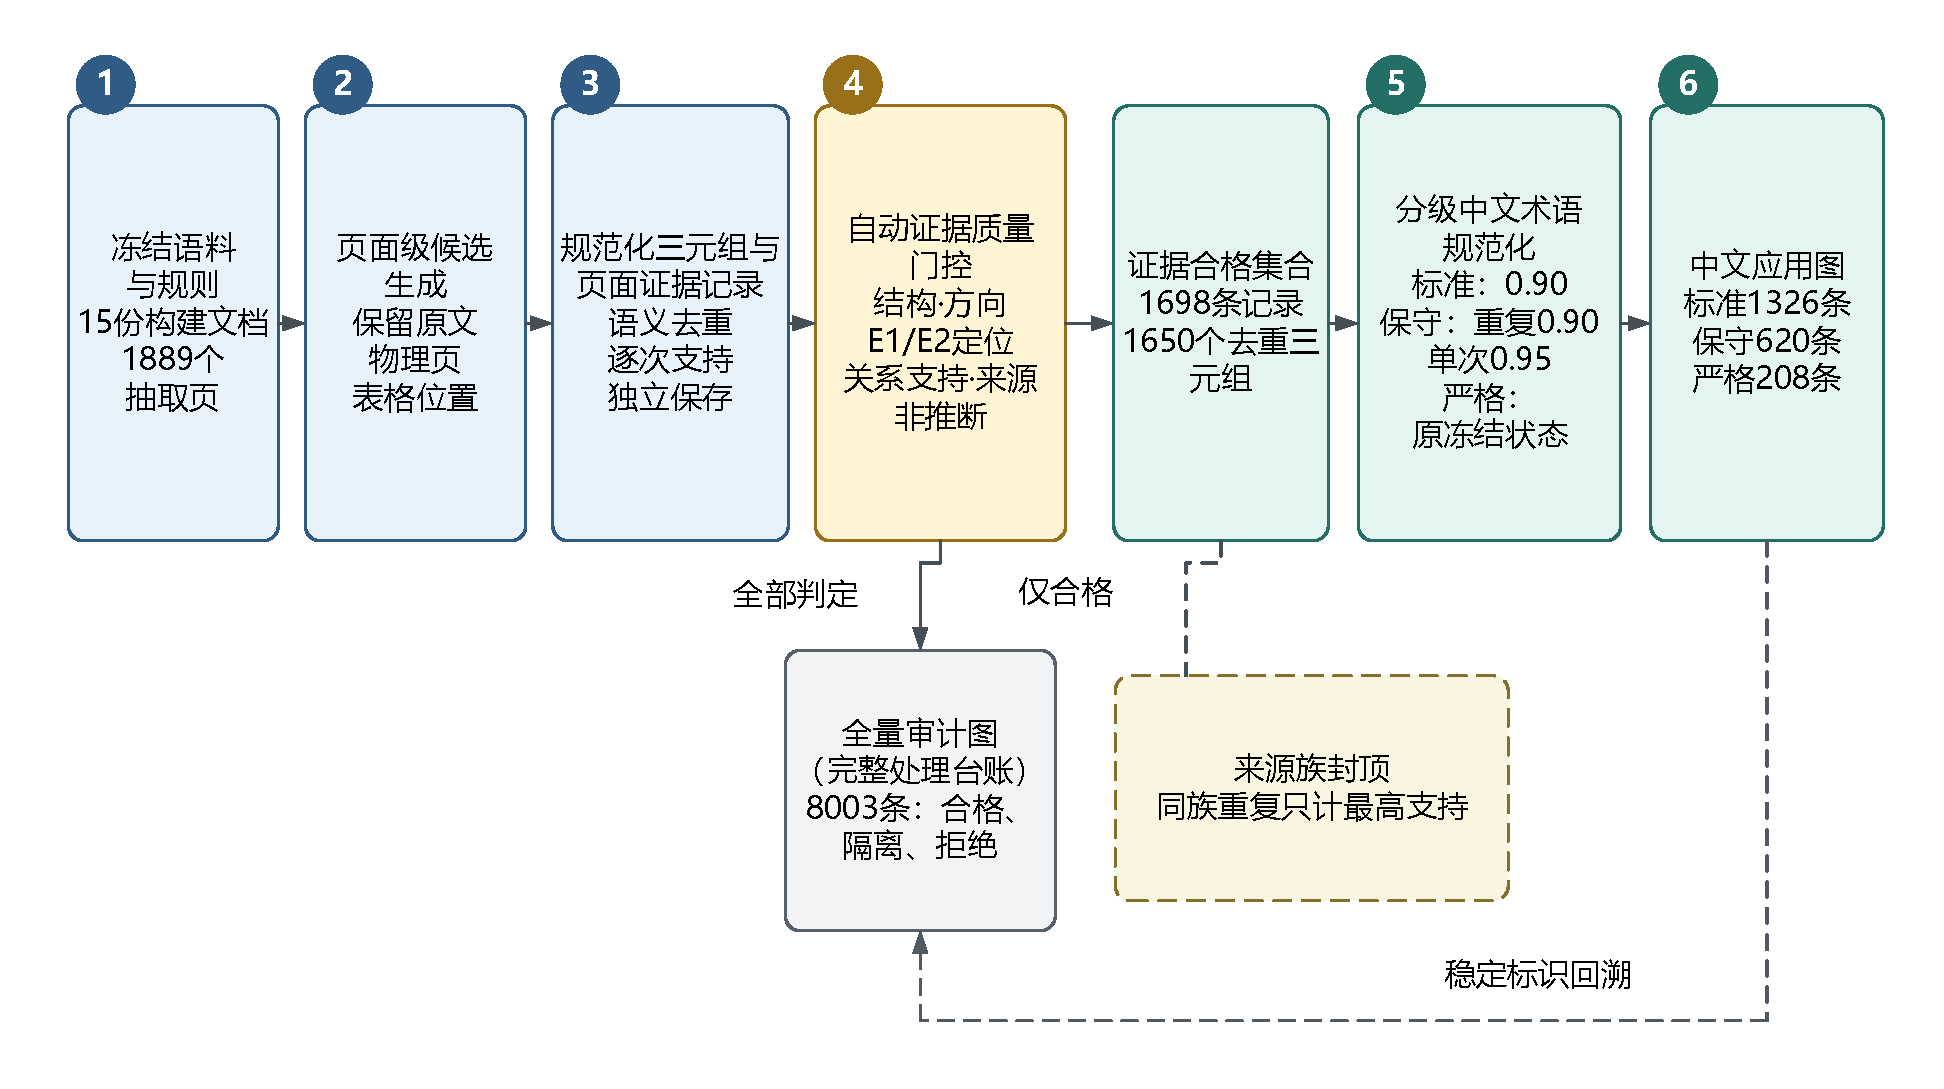
\includegraphics[width=0.90\textwidth]{RP1_ICSMD2026_method_flowchart_zh.pdf}%
  }{\fbox{\parbox[c][35mm][c]{0.94\textwidth}{\centering 流程图待由同目录 Visio 原图导出}}}
  \caption{自动证据质量门控、完整处理台账与分层中文应用图流程}
  \label{fig:pipeline}
\end{figure*}

\subsection{全量审计图与分层中文应用图}

为便于区分，本文将保存全部候选、检查结果和失败原因的图结构称为全量审计图，它相当于可查询的处理台账；将其中满足证据和术语条件的子图称为中文应用图，供检索、展示和后续应用使用。应用图先选取证据合格且非推断的记录，再依据两个端点的中文术语状态划分为标准层、保守层和严格层。标准层用于常规检索和图谱展示，保守层与严格层作为可筛选子集，用于风险较高的查询。各层记录均可通过稳定标识返回全量审计图和原始物理页。完整流程如图\ref{fig:pipeline}所示。

中文术语规范化不改写原文证据。冻结词典和已完成双提示核验的术语直接保留；其余端点只有在中文候选完整、同一实体类型与来源词形不存在名称冲突、受保护字符串完整保留且置信度达到阈值时才进入应用图。标准层统一采用0.90阈值；保守层对重复出现端点采用0.90，对单次出现端点采用0.95；严格层沿用原有词典和双提示核验状态。型号、单位、API、ISO和NPSH等受保护字符串必须保留。新增术语仅表示通过本地一致性和完整性规则，不表示独立模型或领域专家确认。

\subsection{来源族封顶}

同一发布者的多个版本手册可能共享内容。本文以发布者或明确的文档家族定义来源族。对于规范化三元组$c$，每个来源族只保留最高证据分数：
\begin{equation}
s_f(c)=\max_{a_i\in A_f(c)}q_i,\quad
S_{fam}^{(B)}(c)=\frac{1}{B}\sum_{j=1}^{\min(B,|F_c|)}s_{(j)}(c).
\label{eq:family}
\end{equation}
同一来源族内增加重复文档不会增加该族的贡献。来源族只是文档依赖性的工程代理，不是统计独立性证明。

\section{实验与结果}

\subsection{实验设置}

实验包括六部分：全量构图与门控；全部候选的页面定位和来源复核；发布规则故障注入；固定页面上的提示规则与成本比较；全量中文术语规范化与分层应用图比较；来源留出、同族复制和故障知识路径评价。全量复核、故障注入和术语分层实验均在本地执行，不使用人工事实标签；术语分层实验也未向外部模型发送文档片段。输入候选、图谱结构规范和物理页文件的SHA-256写入实验清单。

\subsection{全候选复核与规则故障注入}

8003条候选来自15份构建文档，共引用922个不同物理页。复核程序重新加载物理页对象，不读取候选原有的通过标签。检查内容包括文档与页码映射、文档和页面哈希、URL、发布者、来源族、证据跨度、两个实体位置，以及E2表格单元格、行组和边界框。

表\ref{tab:audit}给出分层结果。1698条证据合格记录全部通过页面、证据、双端点、来源和关系类型检查。881条隔离记录的证据和双端点仍可定位，其中551条通过定位、来源和关系类型检查；其余330条为E3重构证据。5424条拒绝记录中，3947条仍能定位证据，2647条能够同时定位两个实体，1707条通过上述子项检查。拒绝记录仍可能因关系支持、分数或其他规则失败。证据可定位是发布的必要条件，不是充分条件。

\begin{table}[t]
\caption{全候选页面定位与来源复核}
\label{tab:audit}
\centering
\fontsize{7.5}{8.5}\selectfont
\begin{tabular}{lrrrr}
\toprule
决策组 & 记录数 & 证据定位 & 双端点定位 & 子项通过 \\
\midrule
证据合格 & 1698 & 100.00\% & 100.00\% & 100.00\% \\
隔离     & 881  & 100.00\% & 100.00\% & 62.54\% \\
拒绝     & 5424 & 72.77\%  & 48.80\%  & 31.47\% \\
\bottomrule
\end{tabular}
\end{table}

故障注入以1698条复核通过的记录为基线。每次只破坏一项已声明的发布规则。10种故障覆盖哈希与来源、页面与证据定位、关系端点类型和表格结构。共生成13729个有效扰动样本，全部触发至少一项规则失败，见表\ref{tab:mutation}。该实验验证检查器对已编码规则的响应，不代表一般语义错误检出率。

\begin{table}[t]
\caption{发布规则故障注入结果}
\label{tab:mutation}
\centering
\fontsize{7.5}{8.5}\selectfont
\begin{tabular}{llrr}
\toprule
故障组 & 具体故障 & 注入数 & 检出率 \\
\midrule
身份与来源 & 哈希、URL、来源族 & 6792 & 100.00\% \\
页面与证据 & 页码、证据、端点 & 4943 & 100.00\% \\
结构类型   & 关系尾实体类型   & 1698 & 100.00\% \\
表格结构   & 单元格ID、边界框 & 296  & 100.00\% \\
\midrule
合计       & 10种故障         & 13729 & 100.00\% \\
\bottomrule
\end{tabular}
\end{table}

\subsection{全量构图、术语分层与门控贡献}

模型生成8071条原始候选。规范化和去重后得到8003条审计记录，其中1698条证据合格、881条隔离、5424条拒绝。1698条证据记录对应1650个去重规范化三元组和2613个源语言实体。

\begin{table*}[!t]
\caption{中文术语分层规则对应用图规模和知识路径密度的影响}
\label{tab:tiers}
\centering
\footnotesize
\begin{tabularx}{\textwidth}{l>{\raggedright\arraybackslash}Xrrrrrr}
\toprule
应用层 & 术语规则 & 证据记录 & 去重三元组 & 中文实体 & 路径覆盖 & 平均答案数 & 平均证据数 \\
\midrule
严格层 & 原冻结词典及双提示状态 & 208  & 203  & 281  & 34/40 & 5.075 & 6.150 \\
保守层 & 重复端点0.90、单次端点0.95 & 620  & 590  & 870  & 34/40 & 5.575 & 6.800 \\
标准层 & 全部端点统一0.90 & 1326 & 1281 & 2022 & 34/40 & 6.400 & 7.700 \\
\bottomrule
\end{tabularx}
\end{table*}

关系支持方式存在差异。784条记录由E1显式关系词确认，98条由E2表格结构确认，合计882条显式规则支持记录。另有816条依赖同一模型的双提示一致性。后者不是独立模型验证，发布时单独标记。

在固定8003条候选上顺序加入规则后，图谱结构和关系端点类型检查筛除1292条；E1/E2证据定位筛除4206条；关系支持检查筛除801条；0.8分数阈值筛除6条。证据定位和关系支持是主要筛选环节。术语处理扩展后，原严格规则排除的1490条记录中有1118条进入标准应用层，其证据合格状态和页面溯源信息均未改变。

全量术语实验保持1698条证据合格判定不变，只处理中文端点名称。表\ref{tab:tiers}给出三个应用层。标准层覆盖证据合格记录的78.09\%。与严格层相比，标准层增加1118条证据记录、1078个去重三元组和1741个中文实体，记录规模扩大为6.38倍。另有372条证据合格记录因中文名称缺失、冲突、置信度不足或受保护字符串不完整，未进入标准层。只接受重复词形一致且置信度不低于0.90时，应用层包含237条记录、216个去重三元组和301个实体。

标准层和保守层的36项发布检查均无阻断。系统另报告1项警告，来自40条缺少原文的拒绝记录，不影响应用层。证据治理分数0.80与中文候选置信度0.90/0.95作用于不同阶段，前者决定证据是否合格，后者仅决定中文应用层级。

分数阈值由0.80提高至0.85、0.90、0.925、0.95和0.975时，证据合格记录依次为1698、1678、1525、895、867和36条，如图\ref{fig:threshold}所示。阈值达到0.975时，只有8类故障仍满足预定义证据覆盖要求。本文采用0.80作为冻结的工程折中，该阈值不是通过人工真值标签优化得到的统计参数。

\begin{figure}[t]
\centering
\begin{tikzpicture}
\begin{axis}[
  width=0.96\columnwidth,
  height=0.61\columnwidth,
  xlabel={治理分数阈值},
  ylabel={证据合格记录数},
  xmin=0.795, xmax=0.980,
  ymin=0, ymax=1900,
  xtick={0.800,0.850,0.900,0.925,0.950,0.975},
  xticklabel style={font=\scriptsize,rotate=25,anchor=east},
  yticklabel style={font=\scriptsize},
  label style={font=\scriptsize},
  grid=major,
  grid style={draw=gray!30,dashed},
  axis line style={black},
  tick align=outside,
  nodes near coords,
  every node near coord/.append style={font=\scriptsize,anchor=south},
]
\addplot[color={rgb,255:red,45;green,111;blue,176},mark=*,thick]
coordinates {(0.800,1698) (0.850,1678) (0.900,1525) (0.925,895) (0.950,867) (0.975,36)};
\end{axis}
\end{tikzpicture}
\caption{治理分数阈值对证据合格记录数的影响}
\label{fig:threshold}
\end{figure}

\subsection{固定页面提示规则与成本}

提示对照使用相同的20个证据富集页面，并统一模型、温度参数、JSON输出和重试策略。B0为自由抽取；B1加入节点和关系约束；B2增加E1/E2证据要求；B3增加方向和适用范围；Ours使用完整页面级规则。历史实验没有统一最大候选条数和输出token上限，因此表\ref{tab:prompt}只比较当前配置下的规则合格产出和成本，不比较事实准确率。

\begin{table}[H]
\caption{固定页面提示规则及token成本}
\label{tab:prompt}
\centering
\fontsize{7.5}{8.5}\selectfont
\begin{tabular}{lrrrrr}
\toprule
方法 & 原始 & 合格 & 合格/原始 & token/合格 & 合格/10万token \\
\midrule
B0   & 162 & 0   & 0.00\%  & --     & 0.0 \\
B1   & 312 & 50  & 16.03\% & 3565.3 & 28.0 \\
B2   & 226 & 31  & 13.72\% & 5238.0 & 19.1 \\
B3   & 254 & 32  & 12.60\% & 5329.8 & 18.8 \\
Ours & 367 & 148 & 40.33\% & 1466.7 & 68.2 \\
\bottomrule
\end{tabular}
\end{table}

Ours得到148条证据合格记录，是B1的2.96倍。该倍数表示非预算匹配配置下的规则合格产出差异，不表示知识质量提高2.96倍。Ours的总token消耗最高，但每条证据合格记录的token消耗最低。B0没有产生能够直接进入后处理流程的记录，主要原因是自由格式输出与白名单不一致；这不说明B0提出的语义陈述全部错误。

\subsection{来源留出、同族复制与知识路径}

方法、图谱结构规范、阈值和主图冻结后，MP010--MP013在隔离目录中首次执行候选抽取。4份文档共103个物理页，确定性排除后保留94个抽取页。流程生成287条审计记录，其中81条证据合格。81条记录的页面定位率和来源完整率均为100\%。留出文档没有回流主图，也没有用于调参。4份文档均来自MAIB来源族，该实验不能评价来源族多样性或外部事实准确率。

真实语料中有3个完全相同的规范化三元组同时出现在两份文档中，且都属于同一来源族。复制压力测试将证据复制为1、2、4和8份。来源族封顶指数均值始终为0.461058，最大绝对变化为0。按文档直接累加的基线均值则由0.461877升至0.922116，分数不低于0.8的规范化三元组由3个增至1650个。来源族封顶实现了“同族复制不增加支持”。真实语料没有跨来源族的完全相同三元组，本文未验证跨族区分效度。

三个中文应用层均覆盖34/40项预定义路径，覆盖率为85.00\%，四类路径仍分别为7/10、10/10、7/10和10/10。与严格层相比，标准层的平均答案数由5.075增至6.400，平均证据记录数由6.150增至7.700，平均文档数由2.700增至3.075，平均来源族数由2.350增至2.600。术语扩展提高了同一路径下的知识和证据密度，但没有增加路径类型覆盖。该指标不是问答准确率或诊断准确率。

\section{讨论}

\subsection{发布含义、术语分层与人工审核边界}

全候选复核表明，1698条证据合格记录能够重新定位到具体物理页，证据、实体和来源字段形成闭合链路。故障注入表明，删除证据、篡改页码或哈希、破坏实体类型或表格位置后，记录会退出证据合格集合。“证据合格”由可重复执行的规则定义，不是仅靠命名形成的标签。

原208条记录反映的是严格术语状态的覆盖范围，并非证据门控后的图谱总规模。将术语处理扩展到全部证据合格端点后，标准应用层增至1326条，且发布约束未出现阻断。规模增加来自中文术语覆盖扩展，而不是放宽证据质量规则。标准层适合常规检索；保守层和严格层可用于风险较高的查询。

自动门控检查记录是否满足预先声明的文档证据条件。它不判断来源手册是否绝对正确，也不判断现实设备是否必然符合该陈述。本文把可重复的检查要求前置到图谱结构、证据规则、来源族和术语状态中，发布阶段不以专家逐条批准为前置条件。人的作用没有被取消。领域人员仍需确定关系类型、文档范围、证据规则和术语表。冲突记录、安全关键陈述和规则无法处理的条件范围仍可进行定向复核。

\subsection{关系支持方式与测量知识关联}

882条记录的关系由显式关系词或表格角色直接支持。816条记录依赖同一模型的双提示一致性。抽取和判断共享模型参数，错误可能相关。两组记录不能视为强度相同的独立验证结果。普通检索可同时使用两组记录并显示支持方式；安全关键查询可优先使用显式规则支持记录，或对模型一致性支持记录进行定向复核。

本文位于测量与诊断流程的知识数据处理层，不提出新传感器、特征提取算法或故障分类器。中文应用图把压力、流量、振动、温度和电流等测量现象连接到文档中的故障原因、检查动作和维护要求，并保留页面依据。这类知识可用于后续证据检索、诊断辅助或GraphRAG。本文没有使用传感器时序数据，也没有评价故障识别率。

\subsection{局限性}

本研究有六项主要限制。第一，没有领域专家事实标签，不能报告三元组Precision、Recall或F1。第二，816条关系支持记录及新增中文术语候选均依赖抽取模型的输出，可能存在相关误差。第三，故障注入只覆盖已编码的结构、定位和来源错误，不能代表所有语义错误。第四，20页提示对照没有统一候选数量和token上限，只能说明当前配置下的产出和成本。第五，真实语料中没有跨来源族的完全相同三元组，来源族实验只验证同族复制不变性。第六，标准应用层的中文名称只通过本地一致性和完整性规则，未经过独立模型或领域专家的语义核验；另有372条证据合格记录尚未满足标准层的术语条件。

\section{结论}

本文提出面向船舶机舱泵系技术文档的自动证据质量门控方法。规范化三元组与页面证据分层保存，结构、方向、定位、关系支持、来源、语料边界和非推断规则共同决定记录通过、隔离或拒绝。全量审计图保留所有处理结果，中文应用图形成标准、保守和严格三个术语层级。

15份构建文档共产生8003条审计记录和1698条证据合格记录。标准层包含1326条证据记录、1281个去重三元组和2022个中文实体，覆盖证据合格集合的78.09\%。全部证据合格记录均通过重新定位和来源复核，13729个受控规则故障均被检出。81条来源留出记录表明冻结规则能够继续执行，同族复制测试表明来源族封顶不随文档复制增加支持分数。应用层扩展保持34/40的路径覆盖并提高证据密度。上述结果验证的是自动门控、页面级溯源和同源重复控制，不代表客观事实正确率或下游诊断性能。

\section*{致谢与声明}

\textbf{数据可用性：}代码、配置、实验脚本和可公开的派生结果将在论文录用后发布；受版权保护的原始PDF不再分发。\textbf{基金与利益冲突：}本研究未获得外部基金资助，作者声明不存在利益冲突。\textbf{伦理：}本研究不涉及人体、动物或个人隐私数据。\textbf{生成式AI使用：}候选生成、同模型关系检查和中文术语建议通过DashScope API调用阿里云百炼Model Studio中的\mbox{qwen3.7-max}别名完成，调用时间为2026年7月26日至27日。接口只返回模型别名；提示版本、请求标识和响应均已保留。生成式AI也用于中英文语言整理。作者已审阅全文并对论文内容负责。

\bibliographystyle{IEEEtran}
\bibliography{RP1_ICSMD2026_references_v5}

\end{document}
